\section{Simultaneous Connect}
\begin{frame}{Simultaneous Connect}
  \begin{itemize}
    \item Multiple startup
    \item Multiple connect
  \end{itemize}
\end{frame}

\begin{frame}{Simultaneous Connect}
\framesubtitle{Model Performance}
  \begin{figure}[ht]
  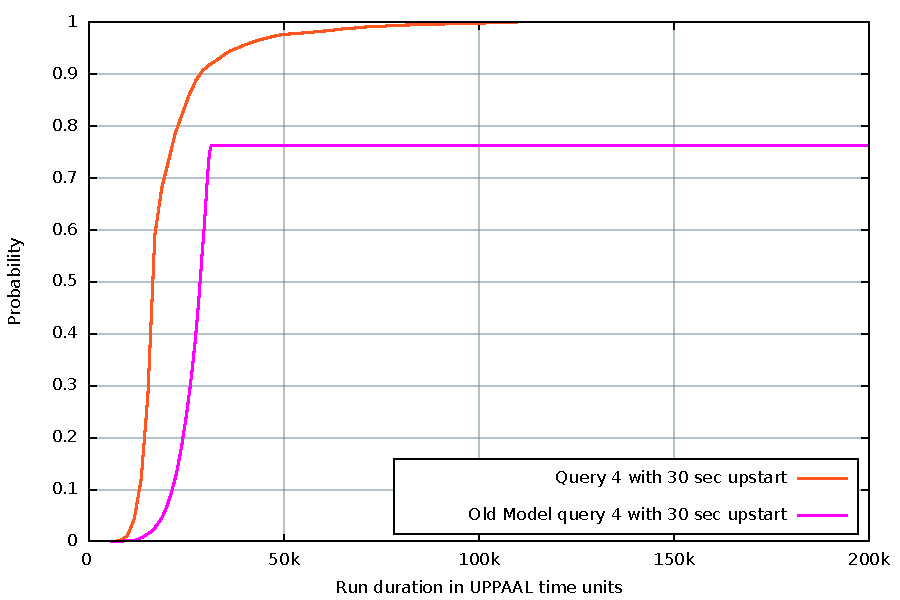
\includegraphics[width=0.9\textwidth]{images/graph.pdf} 
\caption{Graph comparing multiple startup solution to CCRC solution.}
\label{fig:ConnectQueryTime}
\end{figure}
\end{frame}

\section{CCUC}
\subsection{CCUC Assumptions}
\begin{frame}{CCUC assumptions}
The CCUC-problem describes a completely connected graph but in this scenario there is not a guarantee that the transmission will be received; all devices are still in the range of each other.
\end{frame}

\subsection{CCUC Solution}
\begin{frame}{CCUC Improvements}
\framesubtitle{Message Redundancy}

  \begin{itemize}
    \item Pros
      \begin{itemize}
    	\item Increases reliability
    	\item Simple to implement
  	  \end{itemize}
    \item Cons
      \begin{itemize}
    	\item Time consuming
    	\item Naïve solution
  	  \end{itemize}
  \end{itemize}
\end{frame}

\begin{frame}{CCUC Improvements}
\framesubtitle{Results}
\begin{figure}%{\linewidth}
\centering
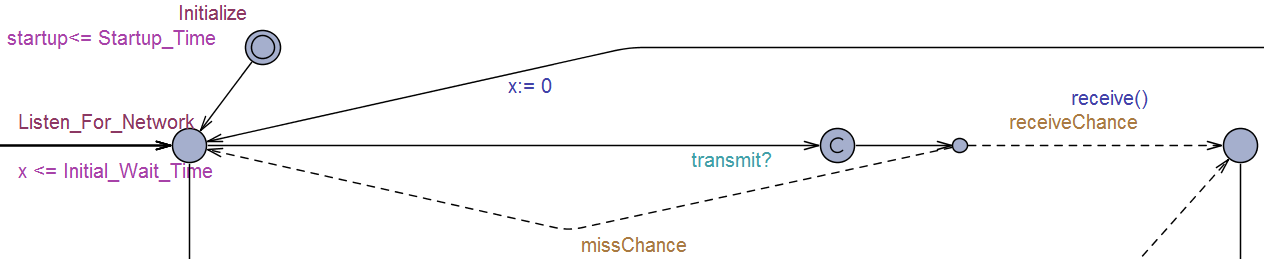
\includegraphics[width=1\textwidth]{images/ccuc.png} 
\end{figure}	
\end{frame}

\begin{frame}{CCUC Improvements}
\framesubtitle{UPPAAL}
\begin{figure}%{\linewidth}
\centering
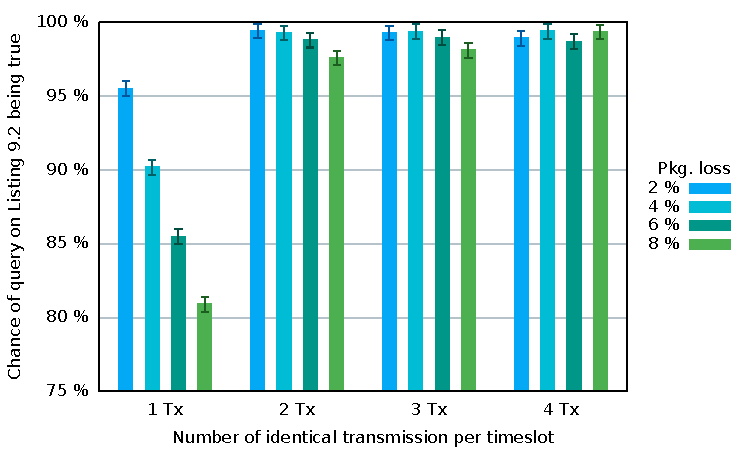
\includegraphics[width=1\textwidth]{images/graph2.pdf} 
\end{figure}
\end{frame}

\begin{frame}{CCUC Improvements}
\framesubtitle{Likely Real World Scenario}

\pgfdeclarelayer{foreground}
\pgfdeclarelayer{background}
\pgfsetlayers{background,main,foreground}

\begin{figure}
\centering
\begin{tikzpicture}  [
        node distance = 1 cm, 
        vertex/.style = {circle, draw, fill=blue!10}, 
        label/.style = {fill=white},
        edge/.style = {draw, -stealth, shorten >= 1pt},
        block/.style = {rectangle, draw, fill=orange, minimum height = 5.5mm, minimum width = 18mm}
    ]

    \node[draw=none](0){};
    \node[vertex, above =     of 0]   (2) {$v_1$};
    \node[vertex, right = 2cm of 0]   (3) {$v_2$};
    \node[vertex, below =     of 0]   (4) {$v_3$};
    
    \path[edge] (2) edge[bend left=14] node [label] {0.85} (3);
    \path[edge] (2) edge[bend left=21] node [label, fill=orange] {0.57} (4);
    \path[edge] (3) edge[bend left=14] node [label] {0.89} (2);
    \path[edge] (3) edge[bend left=14] node [label] {0.93} (4);
    \path[edge] (4) edge[bend left=22] node [label, fill=orange] {0.48} (2);
    \path[edge] (4) edge[bend left=14] node [label] {0.87} (3);
    \begin{pgfonlayer}{background}
    \node[block,  below = 8.5mm of 2]   (1) {};
    \end{pgfonlayer}

\end{tikzpicture}
\end{figure}
\end{frame}
